%-------------------------------------------------------------------------------
%	PACKAGES AND OTHER DOCUMENT CONFIGURATIONS
%-------------------------------------------------------------------------------

\documentclass[twoside,twocolumn]{article}

\usepackage{blindtext} % Package to generate dummy text throughout this template

\usepackage[sc]{mathpazo} % Use the Palatino font
\usepackage[T1]{fontenc} % Use 8-bit encoding that has 256 glyphs
\linespread{1.05} % Line spacing - Palatino needs more space between lines
\usepackage{microtype} % Slightly tweak font spacing for aesthetics

\usepackage[english]{babel} % Language hyphenation and typographical rules

\usepackage[hmarginratio=1:1,top=32mm,columnsep=20pt]{geometry} % Document margins
\usepackage[hang, small,labelfont=bf,up,textfont=it,up]{caption} % Custom captions under/above floats in tables or figures
\usepackage{booktabs} % Horizontal rules in tables

\usepackage{lettrine} % The lettrine is the first enlarged letter at the beginning of the text

\usepackage{enumitem} % Customized lists
\setlist[itemize]{noitemsep} % Make itemize lists more compact

\usepackage{abstract} % Allows abstract customization
\renewcommand{\abstractnamefont}{\normalfont\bfseries} % Set the "Abstract" text to bold
\renewcommand{\abstracttextfont}{\normalfont\small\itshape} % Set the abstract itself to small italic text

\usepackage{titlesec} % Allows customization of titles
\renewcommand\thesection{\Roman{section}} % Roman numerals for the sections
\renewcommand\thesubsection{\roman{subsection}} % roman numerals for subsections
\titleformat{\section}[block]{\large\scshape\centering}{\thesection.}{1em}{} % Change the look of the section titles
\titleformat{\subsection}[block]{\large}{\thesubsection.}{1em}{} % Change the look of the section titles

\usepackage{fancyhdr} % Headers and footers
\pagestyle{fancy} % All pages have headers and footers
\fancyhead{} % Blank out the default header
\fancyfoot{} % Blank out the default footer
\fancyhead[C]{Deep Learning Seminar $\bullet$ Jan 27, 2021$\bullet$ Deep Reinforcement Learning} % Custom header text
\fancyfoot[RO,LE]{\thepage} % Custom footer text

\usepackage{titling} % Customizing the title section

\usepackage{hyperref} % For hyperlinks in the PDF

\usepackage{graphicx}
\usepackage{amsmath}

\usepackage{csquotes}
\usepackage[
    backend=bibtex,
    style=numeric,
]{biblatex}
\addbibresource{multib.bib}

%-------------------------------------------------------------------------------
%	TITLE SECTION
%-------------------------------------------------------------------------------

\setlength{\droptitle}{-4\baselineskip} % Move the title up

\pretitle{\begin{center}\Huge\bfseries} % Article title formatting
\posttitle{\end{center}} % Article title closing formatting
\title{Deep Reinforcement Learning \\ Actor-Critic and Trust region-based} % Article title
\author{%
\textsc{Andres Becker} \\[1ex] % Your name
\normalsize Technische Universität München \\ % Your institution
\normalsize Fakultät für Mathematik
}
%\date{\today} % Leave empty to omit a date
\date{January 27, 2021}
\renewcommand{\maketitlehookd}{%
\begin{abstract}
\noindent
In recent years, significant progress has been made in solving challenging problems across several fields using Reinforcement Learning (RL). Projects like Deep Mind's AlphaGo Zero \cite{silver2017mastering} have accomplish outstanding results without supervised learning on human knowledge, and showed us the amazing results that RL can achieve. In this small resume, we will focus in a group of RL methods called \emph{Actor-Critic} and the \emph{trust region-based} technique aimed to improve their stability.
\end{abstract}
}

%----------------------------------------------------------------------------------------

\begin{document}

% Print the title
\maketitle

%-------------------------------------------------------------------------------
%	ARTICLE CONTENTS
%-------------------------------------------------------------------------------

\section{What is Reinforcement Learning?}
\lettrine[nindent=0em,lines=3]{W}e refer as Machine learning (ML) to the group of algorithms that improve (learn) automatically through experience. Among this algorithms, we could say that there are three main classes (which depend on the kind of experience we provide):
\begin{itemize}
  \item \textbf{Supervised Learning}: The experience is given in the form of input and output examples, and the goal is to learn a general rule that maps inputs to outputs.
  \item \textbf{Unsupervised Learning}: The experience is given in the form of data (no outputs provided) and the goal is to discover hidden patterns in data
  \item \textbf{Reinforcement Learning}: No experience (data) is provided, instead a dynamic \emph{environment} is provided and an \emph{agent} must learn how to interact with it in order to achieve a goal.
\end{itemize}

\noindent In RL an agent interacts with and environment (assumed to be unknown), which in return may provides the agent with a rewards (see figure \ref{fig:RL_interaction}). The agent should take actions so the cumulative rewards is maximized. Ultimately, the goal of RL is that the agent learns a good (optimal) strategy from experimental trials and a relative simple received feedback, so his future rewards is maximized. In reality, the scenario could be a bot playing a game to achieve high scores, or a robot trying to complete physical tasks with physical items.

\begin{figure}
  \centering
  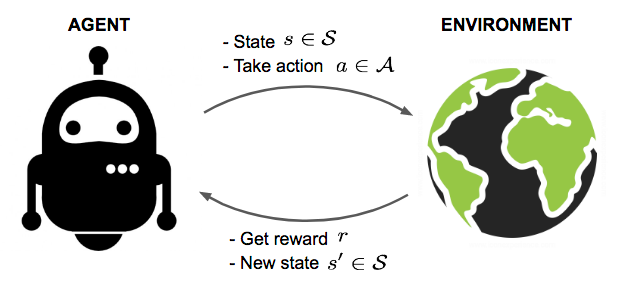
\includegraphics[scale=.24]{Images/RL_illustration.png}
  \caption{Interaction between an Agent and the environment. Image source: \cite{RLsummarylilian}.}
  \label{fig:RL_interaction}
\end{figure}

%------------------------------------------------

\section{Key Concepts of RL}

As we can see in figure \ref{fig:RL_interaction}, the agent interacts with the environment sequentially. Therefore, on time step $t \in \{1,...,T\}$, the agent observe the state of the environment $s_t \in \mathcal{S}$, acts in consequence executing the action $a_t \in \mathcal{A}$, receive its reward $r_t \in \mathcal{R}$ from the environment and observes the new state $s_{t+1} \in \mathcal{S}$.
The tuple $(s_t, a_t, r_t, s_{t+1})$ is known as \emph{transition} step.
This interactions continues until the agent: \textit{i}) completes the task successfully; \textit{ii}) fail or a time limit is reached. This chain of transition steps from the beginning ($t=1$) until the end ($t=T$) is call \emph{Episode}.
We are interested in environments for which the model that defines them is unknown (\emph{Model-free RL}), and has to be learned explicitly as part of the algorithm (otherwise the optimal solution can be found by means of \emph{Dynamec Programming} (DP)).

\noindent This interaction  is an example of a Markov Decision Process (MDP)\cite{Sutton1998} $\mathcal{M}=(\mathcal{S}, \mathcal{A}, P, R)$, where:

\begin{itemize}
    \item $\mathcal{S}$ is the set of states that holds the Markov property\footnote{The conditional probability distribution of future states (conditional on both past and present states) depends only upon the present state, not on the sequence of events that preceded it, i.e. $P(s_{t+1}|s_{t}, s_{t-1},\dots, s_1)=P(s_{t+1}|s_{t})$.}.
    \item $\mathcal{A}$ is the set of actions.
    \item $P$ is the transition probability function: $P(s_{t+1},r_{t+1}|s_t, a_t)$.
    \item $R$ is the reward function: $R(s_t, a_t):=\mathbb{E}[R_{t+1}|s_t,a_t]=\sum_{r\in \mathcal{R}}r \sum_{s' \in \mathcal{S}}P(s',r|s_t, a_t)$.
\end{itemize}

However, note that in fact we are not interested in maximizing the reward on each time step, but the \emph{cumulative reward} in the long run instead. Also, we must think about time as a valuable resource, since in practices we would like to finish a task as soon as possible. This cumulative reward is called \emph{Return} and is defined as:
\begin{equation}
  G_t := \sum_{k=0}^T \gamma^k R_{t+k+1}
\end{equation}
where $\gamma \in [0,1]$ is the discount factor.

Recall that the ultimate goal of RL is to find an optimal strategy, such that it maximize the Return. However, how to choose such actions that they lead to states with high rewards? The answer is the \emph{Policy} $\pi$. The policy is the functions that defines the agent’s behavior and maps a state $s$ to an action $a$. this function can be either deterministic or stochastic:

\begin{itemize}
  \item \textbf{Deterministic}: $\pi: \mathcal{S} \rightarrow \mathcal{A}$; i.e. $\pi(s)=a$.
  \item \textbf{Stochastic}: $\pi: \mathcal{S} \times \mathcal{A} \rightarrow [0, 1]$; i.e. $\pi(a|s)=P_{\pi}(A=a|S=s)$.
\end{itemize}

Now that we have (more or less) a clear idea of what RL seeks (maximize the return $G$) and how to do it (by finding an optimal policy $\pi$), we need to define a way to quantify how good a state $a$ is (in terms of the return $G$) in a given environment (when we follow a policy $\pi$), and how good an action $a$ is (in terms of the return $G$) when the environment is in state $s$ (when we follow a policy $\pi$). This is done through the \emph{State-value} and \emph{Action-value} functions respectively:
\begin{itemize}
    \item \textbf{State-value}: $V_{\pi}(s):= \mathbb{E}_{\pi}[G_t|s_t=s]$.
    \item \textbf{Action-value}: $Q_{\pi}(s, a):= \mathbb{E}_{\pi}[G_t|s_t=s, a_t=a]$.
\end{itemize}

%------------------------------------------------

\section{Policy Gradient methods}
sdcsfcsf

%------------------------------------------------

\section{Actor-Critic}

As I already mentioned, the ultimate goal of RL is to learn a good policy which maximizes the cumulative reward. There are several ways to do this, for example
in \emph{action-value} methods, we learn the value of actions and then select actions based on their estimated action values \cite{Sutton1998} (as it is done in \textit{Q-learning}). However, in \emph{Actor-Critic} methods we learn the policy directly by maximizing the \emph{Expected Cumulative Reward}, by means of a function which is differentiable w.r.t. its parameters\footnote{In fact \emph{Actor-Critic} methods belong to an even broader category of algorithms called \emph{Policy Gradient} methods.}. Moreover, we can also learn the value function as well.
Therefore, the \emph{Actor} refers to the policy and the \emph{Critic} to the estimate of the value function. In deep RL, both the actor and the critic can be represented by non-linear neural networks function approximators \cite{mnih2016asynchronous}.
We write $\pi(a|s,\boldsymbol{\theta}) = Pr(A_t=a | S_t=s, \boldsymbol{\theta}_t=\boldsymbol{\theta})$ to denote the probability that the action $a$ is taken at time $t$, given that the environment is in state $s$ with parameters $\boldsymbol{\theta}$. In the same way, $\boldsymbol{W}$ denote the parameters of the function used to learn the value function.

We denote the \emph{Expected Cumulative Reward} as $J(\boldsymbol{\theta})$, since we seek to maximize it depending on the parameters of the policy $\pi_{\boldsymbol{\theta}}$. Therefore, we can use \emph{Gradient ascent} in $J$ to maximize the performance of the policy:
\begin{equation}
  \boldsymbol{\theta}_{t+1} = \boldsymbol{\theta}_{t} + \alpha \nabla J(\boldsymbol{\theta}_t)
\end{equation}





%------------------------------------------------

\section{Results}

\begin{table}
\caption{Example table}
\centering
\begin{tabular}{llr}
\toprule
\multicolumn{2}{c}{Name} \\
\cmidrule(r){1-2}
First name & Last Name & Grade \\
\midrule
John & Doe & $7.5$ \\
Richard & Miles & $2$ \\
\bottomrule
\end{tabular}
\end{table}

\blindtext % Dummy text

\begin{equation}
\label{eq:emc}
e = mc^2
\end{equation}

\blindtext % Dummy text

%------------------------------------------------

\section{Discussion}

\subsection{Subsection One}

A statement requiring citation \cite{Sutton1998}.
\blindtext % Dummy text

\subsection{Subsection Two}

\blindtext % Dummy text

%-------------------------------------------------------------------------------
%	REFERENCE LIST
%-------------------------------------------------------------------------------

\printbibliography

%-------------------------------------------------------------------------------

\end{document}
